\problemname{Mineral deposits}

\illustration{.3}{img/turnbull.jpg}{Eroding mud face exposing new minerals. Photo: Michael D.\ Turnbull, licence: CC BY-SA.}

\noindent
You handle signal processing for an extra-terrestrial mining company, and your vessel is currently approaching an asteroid. 
Preliminary scans show the presence of $k$~mineral deposits on the asteroid, but their precise locations are unknown.

\medskip

The surface of the asteroid can be seen as a grid of integer coordinates.
Each of the mineral deposits is located at unknown integer coordinates such that the $i$th deposit has coordinates $(x_i, y_i)$ with  
$-b \le x_i \le b$ and $-b\le y_i \le b$ %constraint:depositcoords
for some integer $b$ corresponding to the size of your initial scan. All locations are unique.

To determine the precise locations of the mineral deposits, you may send probes to the surface of the asteroid. 
The probes are sent out in waves of several probes at once.

Say you sent a wave of $d$~probes to the surface at coordinates $(s_j,t_j)$ for $1\leq j\leq d$.
When a probe arrives at its coordinates, it determines the Manhattan distances to each of the $k$~mineral deposits and sends the distances back to the ship. 
All data packets arrive at the same time, and it is not possible to determine which probes returned which distances. 
Thus the wave returns the $k\cdot d$ integer distances
\[|x_i-s_j| + |y_i - t_j| \qquad\text{for all } i \in \{1,\ldots,k\} \text{ and } j \in\{ 1,\ldots,d\}\,.\]

You need to minimise the number of waves of probes that is sent to the surface.


\section*{Interaction}

This is an interactive problem.
Interaction begins with you reading a single line containing three integers $b$, $k$, and $w$:
the grid's boundary~$b$,
the number~$k$ of mineral deposits,
and the maximum number~$w$ of waves you may send.

You then ask at most $w$ queries, each corresponding to a wave.
A query consists of \texttt{?} followed by $2d$ integers separated by space, such as ``\texttt{?} $s_1$ $t_1$ $\cdots$ $s_d$ $t_d$'', where the number~$d$ of probes in this wave must satisfy
$1\leq d\leq 2000$. % constraint:wavesize
The values $(s_i,t_i)$ are interpreted as the coordinates of the $i$th probe and must satisfy
$-10^8 \leq s_i \leq 10^8$ and $-10^8 \leq t_i \leq 10^8$. % constraint:probecoordinates
Each $(s_i,t_i)$ in a wave must be unique.
The response is a single line with $k \cdot d$ integers in non-decreasing order: 
the Manhattan distances between all pairs of mineral deposits and probe coordinates.
The total number of probes across all waves may not exceed
$2\cdot 10^4.$ % constraint:totalprobes

Interaction ends with you printing a single line consisting of \texttt{!} followed by $k$ points $x_1, y_1, x_2, y_2, \ldots x_k, y_k$, separated by space.
This must be your last line of output.

Your submission is considered correct if you print all locations of the mineral deposits.
You may print them in any order.

\section*{Constraints and Scoring}

We always have 
$1\leq b \leq 10^8$, % constraint:b
$1 \leq k \leq 20$, % constraint:k
and
$2 \le w \le 10^4$. % constraint:w

Your solution will be tested on a set of test groups, each worth a number of points.
Each test group contains a set of test cases.
To get the points for a test group you need to solve all test cases in the test group.
Your final score will be the maximum score of a single submission.

\medskip
\begin{tabular}{lll}
Group & Points & Constraints \\\hline
  $1$ & $16$ & $k = 1, w = 10^4$\\
  $2$ & $19$ & $w \ge 500$\\
  $3$ & $11$ & $w \ge 210$\\
  $4$ & $13$ & $w \ge 130$\\
  $5$ & $14$ & $w \ge 3$, $b \le 10^4$\\
  $6$ & $14$ & $w \ge 3$, $b \le 10^7$\\
  $7$ & $13$ & \emph{No further constraints}
\end{tabular}

\section*{Example}

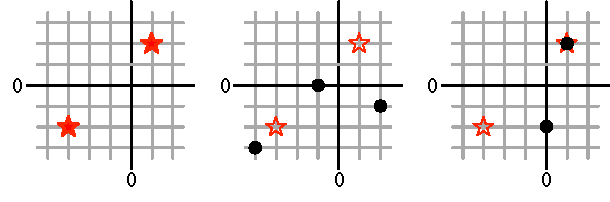
\includegraphics[width=.6\textwidth]{img/sample1.pdf}

In this example, there are $k=2$ mineral deposits at positions $(1,2)$ and $(-3,-2)$, shown as red stars.
In the first wave, you might send $d=3$ probes to $(-4,-3)$, $(-1, 0)$, and $(2,-1)$, shown as black dots.
This wave would return the $6$ distances \[
  2, 4, 4, 4, 6, 10\,.
\]
In the next wave, you might send $d=2$ probes to $(1,2)$ and $(0,-2)$.
This wave would return the $4$ distances \[
  0, 3, 5, 8\,.
\]
